\documentclass[a4paper, 12pt]{article} 

%--------------------------------------
%Russian-specific packages
%--------------------------------------
%\usepackage[warn]{mathtext}
\usepackage[T2A]{fontenc}
\usepackage[utf8]{inputenc}
\usepackage[english,russian]{babel}
\usepackage[intlimits]{amsmath}
\usepackage{esint}
%--------------------------------------
%Hyphenation rules
%--------------------------------------
\usepackage{hyphenat}
\hyphenation{ма-те-ма-ти-ка вос-ста-нав-ли-вать}
%--------------------------------------
%Packages
%--------------------------------------
\usepackage{amsmath}
\usepackage{amssymb}
\usepackage{amsfonts}
\usepackage{amsthm}
\usepackage{latexsym}
\usepackage{mathtools}
\usepackage{epstopdf}
\usepackage{etoolbox}%Булевые операторы
\usepackage{extsizes}%Выставление произвольного шрифта в \documentclass
\usepackage{geometry}%Разметка листа
\usepackage{indentfirst}
\usepackage{wrapfig}%Создание обтекаемых текстом объектов
\usepackage{fancyhdr}%Создание колонтитулов
\usepackage{setspace}%Настройка интерлиньяжа
\usepackage{lastpage}%Вывод номера последней страницы в документе, \lastpage
\usepackage{soul}%Изменение параметров начертания
\usepackage{hyperref}%Две строчки с настройкой гиперссылок внутри получаеммого
\usepackage[usenames,dvipsnames,svgnames,table,rgb]{xcolor}% pdf-документа
\usepackage{multicol}%Позволяет писать текст в несколько колонок
\usepackage{cite}%Работа с библиографией
\usepackage{subfigure}% Человеческая вставка нескольких картинок
\usepackage{tikz}%Рисование рисунков
\usepackage{float}
% Для картинок Моти
\usepackage{misccorr}
\usepackage{lscape}
\usepackage{cmap}
\usepackage{hyperref}
\usepackage{xcolor}



\usepackage{graphicx,xcolor}
\graphicspath{{Pictures/}}
\DeclareGraphicsExtensions{.pdf,.png,.jpg}

%----------------------------------------
%Список окружений
%----------------------------------------
\newenvironment {theor}[2]
{\smallskip \par \textbf{#1.} \textit{#2}  \par $\blacktriangleleft$}
{\flushright{$\blacktriangleright$} \medskip \par} %лемма/теорема с доказательством
\newenvironment {proofn}
{\par $\blacktriangleleft$}
{$\blacktriangleright$ \par} %доказательство
%----------------------------------------
%Список команд
%----------------------------------------
\newcommand{\grad}
{\mathop{\mathrm{grad}}\nolimits} %градиент

\newcommand{\diver}
{\mathop{\mathrm{div}}\nolimits} %дивергенция

\newcommand{\Def}[1]
{\underline{\textbf{#1}}} %определение

\newcommand{\RN}[1]
{\MakeUppercase{\romannumeral #1}} %римские цифры

\newcommand {\theornp}[2]
{\textbf{#1.} \textit{ #2} \par} %Написание леммы/теоремы без доказательства

\newcommand{\qrq}
{\ensuremath{\quad \Rightarrow \quad}} %Человеческий знак следствия

\newcommand{\qlrq}
{\ensuremath{\quad \Leftrightarrow \quad}} %Человеческий знак равносильности

\renewcommand{\phi}{\varphi} %Нормальный знак фи

\newcommand{\me}
{\ensuremath{\mathbb{E}}}

\newcommand{\md}
{\ensuremath{\mathbb{D}}}




%\renewcommand{\vec}{\overline}




%----------------------------------------
%Разметка листа
%----------------------------------------
\geometry{top = 3cm}
\geometry{bottom = 2cm}
\geometry{left = 1.5cm}
\geometry{right = 1.5cm}
%----------------------------------------
%Колонтитулы
%----------------------------------------
\pagestyle{fancy}%Создание колонтитулов
\fancyhead{}
%\fancyfoot{}
\fancyhead[R]{\textsc{ОДУ: Контрольная работа 2}}%Вставить колонтитул сюда
%----------------------------------------
%Интерлиньяж (расстояния между строчками)
%----------------------------------------
%\onehalfspacing -- интерлиньяж 1.5
%\doublespacing -- интерлиньяж 2
%----------------------------------------
%Настройка гиперссылок
%----------------------------------------
\hypersetup{				% Гиперссылки
	unicode=true,           % русские буквы в раздела PDF
	pdftitle={Заголовок},   % Заголовок
	pdfauthor={Автор},      % Автор
	pdfsubject={Тема},      % Тема
	pdfcreator={Создатель}, % Создатель
	pdfproducer={Производитель}, % Производитель
	pdfkeywords={keyword1} {key2} {key3}, % Ключевые слова
	colorlinks=true,       	% false: ссылки в рамках; true: цветные ссылки
	linkcolor=blue,          % внутренние ссылки
	citecolor=blue,        % на библиографию
	filecolor=magenta,      % на файлы
	urlcolor=cyan           % на URL
}
%----------------------------------------
%Работа с библиографией 
%----------------------------------------
\renewcommand{\refname}{Список литературы}%Изменение названия списка литературы для article
%\renewcommand{\bibname}{Список литературы}%Изменение названия списка литературы для book и report
%----------------------------------------
\begin{document}
\begin{center}


\vfill






\textbf{РЕШЕНИЯ ЗАДАЧ ТЕСТОВОГО ВАРИАНТА\\[3mm]
КОНТРОЛЬНОЙ РАБОТЫ №2\\[3mm]
по курсу "Обыкновенные дифференциальные уравнения"
\\
}
\end{center}



	\section*{Вариант IV}
		\subsection* {Задача 1}


 Решить систему дифференциальных уравнений (Задача Коши): 
\begin{equation}
\left\{
\begin{array}{lr}
\dot{x} = 3x-2y\\
\dot{y} = 2x-2y
\end{array}
\right.
, \;\;\;\; x(\cdot)\in \textbf{R},\; y(\cdot)\in \textbf{R}
\label{eq:1}
\end{equation}

\textbf{Решение:} \par
Обозначим 
\[
A = \left(
\begin{array}{cc}
-3 & -2\\
2 & -2\\
\end{array}
\right)\]

(i) Стационарные точки:

\[
\left\{
\begin{array}{lr}
\dot{x} = 0\\
\dot{y} = 0
\end{array}
\right.
\Leftrightarrow (0;0)
\]


(ii) Найдем собственные числа матрицы A:
\[det(A-\lambda \hat{I})=
\begin{vmatrix}
3-\lambda & -2 \\
2 & -2-\lambda
\end{vmatrix}
=0\]

\[\lambda_1=-1, \; \lambda_2=2\]
\\Найдем собственные векторы:
\[\lambda_1=-1,\;\;\;\;\; p^1=
\left(
\begin{array}{cc}
1\\
2\\
\end{array}
\right)
\]



\[\lambda_1=2,\;\;\;\; p^2=
\left(
\begin{array}{cc}
2\\
1\\
\end{array}
\right)
\]
Каноническое преобразование координат:
\[A = S\Lambda S^{-1}\]
\[
S = \left(
\begin{array}{cc}
1 & 2\\
2 & 1\\
\end{array}
\right)\;\;\;\;\;
S^{-1} = \left(
\begin{array}{cc}
-1 & 2\\
2 & -1\\
\end{array}\right)\;\;\;\;\;
\Lambda = \left(
\begin{array}{cc}
-1 & 0\\
0 & 2\\
\end{array}\right)
\]

Система в новых координатах:
\[\left(
\begin{array}{c}
\dot{\alpha}_1\\
\dot{\alpha}_2
\end{array}
\right)=\Lambda\left(
\begin{array}{c}
{\alpha}_1 \\
{\alpha}_2
\end{array}
\right)\]


(iii) Прямые, при пересечении которых фазовые траектории параллельны осям $x$ и $y$.\\
Параллельно оси y:
\[\dot{x} = 3x-2y=0\Leftrightarrow y = 3/2x\]\\
Параллельно оси x:
\[\dot{y} = 2x-2y=0\Leftrightarrow y = x\]
\begin{figure}[H]
	\centering
	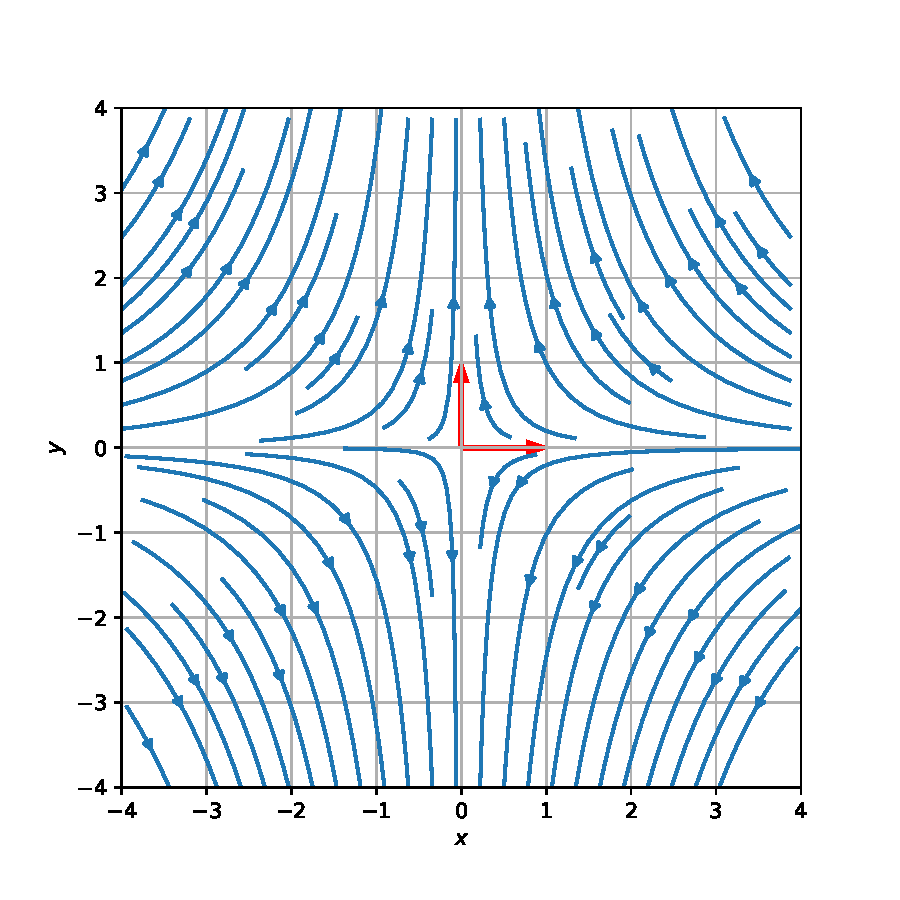
\includegraphics[scale=0.7]{1a1_0}
	\caption{Фазовый портрет в канонических координатах}
	\label{im:1a1_0}
\end{figure}



(iv) Фазовый портрет(\ref{eq:1}) в исходных координатах:

\begin{figure}[H]
	\centering
	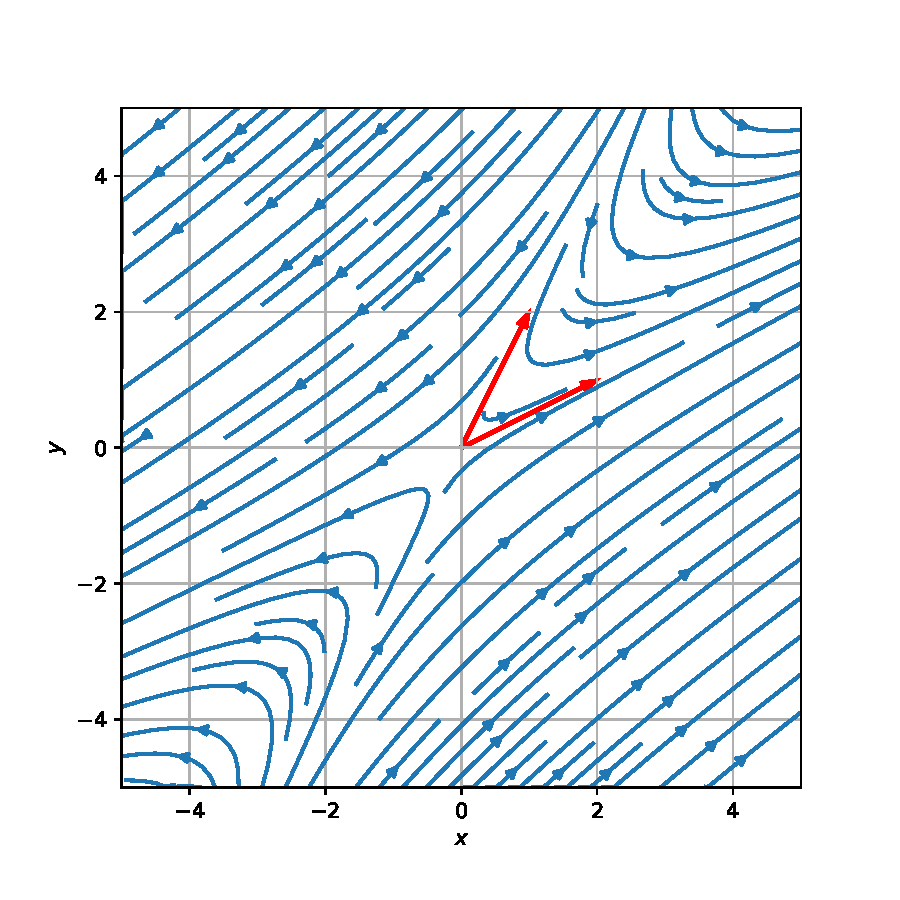
\includegraphics[scale=0.7]{1a1_1}
	\caption{Фазовый портрет в исходных координатах}
	\label{im:1a1_1}
\end{figure}

(v) $\lambda_{1,2}$ разных знаков, картина -- \textbf{седловая точка}.







	\subsection* {Задача 2}
 Решить систему дифференциальных уравнений (Задача Коши): 
\begin{equation}
\left\{
\begin{array}{lr}
\dot{x} = -x+4y+2e^{3t}\\
\dot{y} = -x+3y-2
\end{array}
\right.
, \;\;\;\; x(\cdot)\in \textbf{R},\; y(\cdot)\in \textbf{R}
\label{eq:2}
\end{equation}

\textbf{Решение:} \par
Обозначим 
\[
A = \left(
\begin{array}{cc}
-1 & 4\\
-1 & 3\\
\end{array}
\right)\]

(i) Найти общее решение соответствующей однородной системы.
\[det(A-\lambda \hat{I})=
\begin{vmatrix}
-1-\lambda & 4 \\
-1 & 3-\lambda
\end{vmatrix}
=0\]


\[\lambda =1\;\;\text{-- собственное число кратности 2}\]
Собственный вектор:
\[p=
\left(
\begin{array}{cc}
2\\
1\\
\end{array}
\right)
\]
Пространство векторов имеет размерность 1:
\[\dim \{ p\in \textbf {R}^2: p_1^1=-p_2^1\}=1\]
Собственному числу соответствует одномерное пространство собственных векторов. Найдем присоединенный вектор:\\
\[(A-\lambda \hat{I})v=p\]

\[v=
\left(
\begin{array}{cc}
-1\\
0\\
\end{array}
\right)
\]
Каноническое преобразование координат:
\[A = S\Lambda S^{-1}\]
\[
S = \left(
\begin{array}{cc}
2 & -1\\
1 & 0\\
\end{array}
\right)\;\;\;\;\;
S^{-1} = \left(
\begin{array}{cc}
0 & 1\\
-1 & 2\\
\end{array}\right)\;\;\;\;\;
\Lambda = \left(
\begin{array}{cc}
1 & 1\\
0 & 1\\
\end{array}\right)
\]
Получаем общее решение однородной системы:
\[\left(
\begin{array}{c}
x(t)\\
y(t)
\end{array}
\right)=e^{At}\left(
\begin{array}{c}
C_1 \\
C_2
\end{array}
\right)=Se^{\Lambda}S^{-1}\left(
\begin{array}{c}
C_1 \\
C_2
\end{array}
\right)=e^t
\left(
\begin{array}{cc}
2 & -1 \\
1 & 0
\end{array}
\right)
\left(
\begin{array}{cc}
1 & t \\
0 & 1
\end{array}
\right)
\left(
\begin{array}{cc}
0 & 1 \\
1- & 2
\end{array}
\right)\left(
\begin{array}{c}
C_1 \\
C_2
\end{array}
\right)=\]\[
=e^t
\left(
\begin{array}{cc}
1-2t & 4t \\
-t & 1+2t
\end{array}
\right)\left(
\begin{array}{c}
C_1 \\
C_2
\end{array}
\right)\]
Частное решение будем искать методом неопределенных коэффициентов:
\[x(t)_{\text{частн}}=ae^{3t}+b\]
\[y(t)_{\text{частн}}=ce^{3t}+d\]
Подставляя эти выражения в систему (\ref{eq:2}), получим:
\[
\left\{
\begin{array}{lr}
3ae^{3t}=-(ae^{3t}+b)+4(ce^{3t}+d)+2e^{3t}\\
3ce^{3t}=-(ae^{3t}+b)+3(ce^{3t}+d)-2\\
\end{array}
\right.
\]
Отсюда находим:
\[
\left\{
\begin{array}{lr}
a = 0\\
c = - \frac 1 2 \\
d = -2 \\
b=-8
\end{array}
\right.
\]
Общее решение уравнения есть сумма частного и однородного:

\begin{equation}
x(t) = e^t\left(\left(1-2t\right)C_1+4tC_2\right)-8
\label{eq:3}
\end{equation}
\begin{equation}
y(t) = e^t\left(-tC_1+\left(2t+1\right)C_2\right)-\frac 1 2 e^{3t}-2
\label{eq:4}
\end{equation}

(ii) Найти траекторию системы (\ref{eq:2}), проходящую через начало координат.\\
Подставляя точку $(0;0;0)$ в (\ref{eq:3}) и (\ref{eq:4}), находим константы $C_1$ и $C_2$:

\[C_1 =8\;\;\;\;\; C_2 = \frac 5 2\]

\[
x_0(t) = e^t\left(8-6t\right)-8\]\[
y_0(t) = e^t\left(-3t+\frac 5 2\right)- \frac 1 2 e^{3t} - 2
\]

(iii) Для траектории, найденной в (ii), найти пределы $\lim_{t\rightarrow\pm\infty}y(t)/x(t)$ (если они существуют).


\[\lim_{t\rightarrow+\infty}\frac{e^t\left(-3t+\frac 5 2\right)- \frac 1 2 e^{3t} - 2}{ e^t\left(8-6t\right)-8}=\lim_{t\rightarrow+\infty}\frac{e^t\left(-3+\frac 5 {t2}\right)- \frac 1 2 e^{3t}/t - 2/t}{ e^t\left(8/t-6\right)-8/t}\rightarrow+\infty\]

\[\lim_{t\rightarrow-\infty}\frac{e^t\left(-3t+\frac 5 2\right)- \frac 1 2 e^{3t} - 2}{ e^t\left(8-6t\right)-8}=\frac{1}{4}\]


	\subsection* {Задача 3}
Для дифференциального уравнения 
\begin{equation}
y''+4y=\frac{6}{\sin\;2x}, \;\;\;\; y(\cdot)\in \textbf{R},\; x\in (0, \pi/2)
\label{eq:5}
\end{equation}

(i) Найти общее решение соотвествующего однородного уравнения.\\
Однородное уравнение -- известное уравнение осциллятора. Его решение ищем в виде:
\[y(x) = e^{ax}\]
\[a^2e^{ax}+4e^{ax}=0\]
\[a^2+4=0\]
\[a = \pm 2i\]
Тогда решение:
\[y(x)=C_1e^{ix}+C_2e^{-ix}\]
Воспользуемся формулой Эйлера:
\[y(x)= C_1\sin{2x}+C_2\cos{2x}\]

(ii) Найти общее решение уравнения (\ref{eq:5}).\\
Будем решать уравнение методом вариации постоянной:

\[y(x)= C_1(t)\cos{2x}+C_2(t)\sin{2x}\]
Получили систему:
\[ \left(
\begin{array}{cc}
\sin{2x} & \cos{2x} \\
2\cos{2x} & -2\sin{2x}
\end{array}
\right) \left(
\begin{array}{c}
C_1' \\
C_2'
\end{array} 
\right)= \left(
\begin{array}{c}
0 \\
6/\sin{2x}
\end{array}
\right) \]
Найдем коэффициенты методом Крамера:
\[C_1' = \frac{\begin{vmatrix}
0 & \cos{2x} \\
6/\sin{2x} & -2\sin{2x}
\end{vmatrix}}{\begin{vmatrix}
\sin{2x} & \cos{2x} \\
2\cos{2x} & -2\sin{2x}
\end{vmatrix}}= \frac {6\ctg{2x}}{2} = 3\ctg{2x}\]

\[C_2' = \frac{\begin{vmatrix}
\sin{2x} & 0 \\
2\cos{2x} & 6/\sin{2x}
\end{vmatrix}}{\begin{vmatrix}
\sin{2x} & \cos{2x} \\
2\cos{2x} & -2\sin{2x}
\end{vmatrix}}= \frac {6}{-2} = - 3\]
Находим 
\[C_1 = \frac 3 2 \ln{(\sin{2x})}\]
\[C_2=-3x\]
Тогда общее решение:
\[y(x) = C_1\sin{2x}+C_2\cos{2x}+\frac {3} {2} \ln{(\sin{2x})}\sin{2x}-3x\cos{2x}\]


	\subsection* {Задача 4}

Для дифференциального уравнения
\begin{equation}
\ddot{x}+\dot{x}-x=3t\sin{t}, \;\;\;\; x(\cdot)\in \textbf{R}
\label{eq:6}
\end{equation}

(i) найти общее решение соответствующего однородного уравнения.\\
Характеристическое уравнение для левой части (\ref{eq:6}):
\[a^2+a-1=0\]
\[a_{1,2}=-\frac 1 2 \pm \frac {\sqrt{5}}{2}\]
Тогда общее решение однородного уравнения:
\begin{equation}
x(t) = C_1e^{t\left(-\frac 1 2 - \frac {\sqrt{5}}{2}\right)}+C_2e^{t\left(-\frac 1 2 + \frac {\sqrt{5}}{2}\right)}
\label{eq:7}
\end{equation}

(ii) найти общее решение уравнения (\ref{eq:6}).\\
Частное решение для этой правой части ищем в виде:
\[ x(t) = a\cos{t}+bt\cos{t}+c\sin{t}+dt\sin{t}\]
Поставляя в (\ref{eq:6}), находим коэффициенты: 
\[
\left\{
\begin{array}{lr}
a = -\frac 6 5 \\
c = - \frac 3 5 \\
d =  \frac 3 5 \\
b=- \frac 6 5 
\end{array}
\right.
\]
Суммируя частное и однородное решения, получим ответ:

\[x(t) = -\frac 6 5\cos{t} - \frac 3 5 t \cos{t} + \frac 3 5 \sin{t} - \frac 6 5 t\sin{t} + C_1e^{t\left(-\frac 1 2 - \frac {\sqrt{5}}{2}\right)}+C_2e^{t\left(-\frac 1 2 + \frac {\sqrt{5}}{2}\right)} \]

\end{document}